\documentclass[11pt,a4paper]{article}
    \usepackage{jinstpub}
    \usepackage{floatrow}
    \usepackage{subfig}
    \title{EPD}
    \author[a]{Liang Z.}
    \author[a]{Shen K.}
    \author[a]{Wu Y.}
    \author[a]{Shao M.}
    \affiliation[a]{University of Science and Technology of China, JinZhai Road, HEFEI, China}

    \emailAdd{liangzheng1021@163.com}
    \emailAdd{skfyl@mail.ustc.edu.cn}
    \emailAdd{torrence@mail.ustc.edu.cn}
    \emailAdd{swing@ustc.edu.cn}

    \abstract{%\bf R\mdseries elativistic \bf H\mdseries eavy \bf I\mdseries on \bf C\mdseries ollider(RHIC), which locates at \bf B\mdseries rookhaven 
    % \bf N\mdseries ational \bf L\mdseries ab(BNL), is determined to collide ions. \bf S\mdseries olenoidal \bf T\mdseries racker \bf A\mdseries t \bf R\mdseries HIC(STAR)
    % tracks the thousands of particles produced by ion collisions at RHIC. 
    \emph{E}vent \emph{P}lane, centrality, and trigger \emph{D}etector(EPD) is a plastic scintillation detector
    designed to be installed on RHIC-STAR. SiPMs are used to collect photons produced by scintillators, while FEE boards and RX boards are used to amplify and recieve signals from SiPMs.
    We care about their performances before installing, e.g., UI curve, noise frequency spectrum, signal characters.
    Thus, we setup a batch test system, which is made up of pulse generator, LED, digitizer, etc.
    }

    \keywords{STAR, EPD, SiPM, FEE board, RX board, Noise, Signal, Batch test}
    
    % \notoc
    % \toccontinuoustrue

\begin{document}
\maketitle
\flushbottom

\section{Introduction}
Relativistic Heavy Ion Collider(RHIC), locates at Brookhaven National Lab(BNL), 
is determined to collide heavy ions. The Solenoidal Tracker at RHIC(STAR) tracks
particles produced by RHIC.
\paragraph{STAR}
\paragraph{BESII}
\paragraph{EPD}

\section{System Design}
\paragraph{Test Items \& Test Methods}First, all device's mechanical integrity should be ensured and SiPMs' thickness should be measured,
i.e., we should first check whether there exists any obvious damage and than measure thickness of SiPM by microscope.

Second, UI curve of a SiPM can help us judge its basic electric properties, e.g., dark current and break down(BD) voltage.
Under good dark conditions, we change bias voltage on SiPMs from 50V to 65V, with 0.5V step size. This range covers all what we are interested in.
We can control FEE board and acquire U/I information through computer.

Third, electronic noise can reflect electronic performances. Rib or strange peaks shouldn't appear in noise frequency spectrum. Thus, we set bias voltage on
SiPM at 46.5V, which is below its BD voltage, and output RX board signal into oscilloscope or digitizer to collect waveforms, and finally get frequency spectrum.

Last, several characters of SiPM's signal should be tested. Shape of signal should be normal, and pedestal should be changed when adjusting DAC. In addition, we need check
spectrum of signal charge integral in order to judge the quality of single photon signal's resolution. We first set bias voltage below BD voltage(46.5V) to check pedestal. And
then, set bias voltage at OP voltage(60V) to check integral spectrum, meanwhile, illuminate SiPMs with light from a LED, which is driven by wavefrom generator. Output all signal
into oscilloscope/digitizer, which is triggered in the same frequency as LED. After collecting enough waveforms and a little further processing, we get integral spectrum.

\paragraph{System Chart}
System chart is as shown in figure \ref{fig:System Chart}.

\paragraph{Instrument Selection}It's easy to choose LED, whose luminous wavelength range should cover peak of scintillators' luminescence spectrum, i.e., 475nm.
However, choosing oscilloscope or digitizer is a tough decision. Oscilloscope can help to get more accurate result, but only have 4 input channels. While digitizer have
16 channels but has less precision. Besides, digitizer should be calibrated before using.

\begin{figure}[ht]
    \centering
    \begin{floatrow}
        \centering
        \ffigbox{\caption{System Chart}\label{fig:System Chart}}{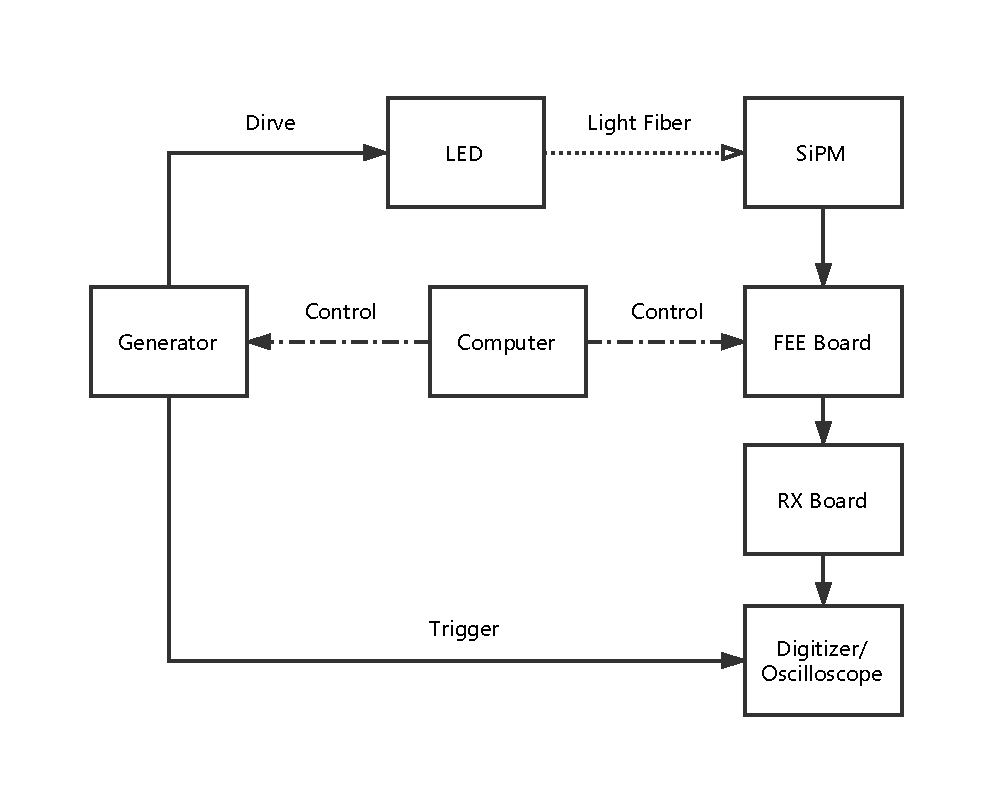
\includegraphics[scale=0.45]{fig/System_Chart.pdf}}
        \centering
        \ffigbox{\caption{UI Curve Example}\label{fig:UI Curve Example}}{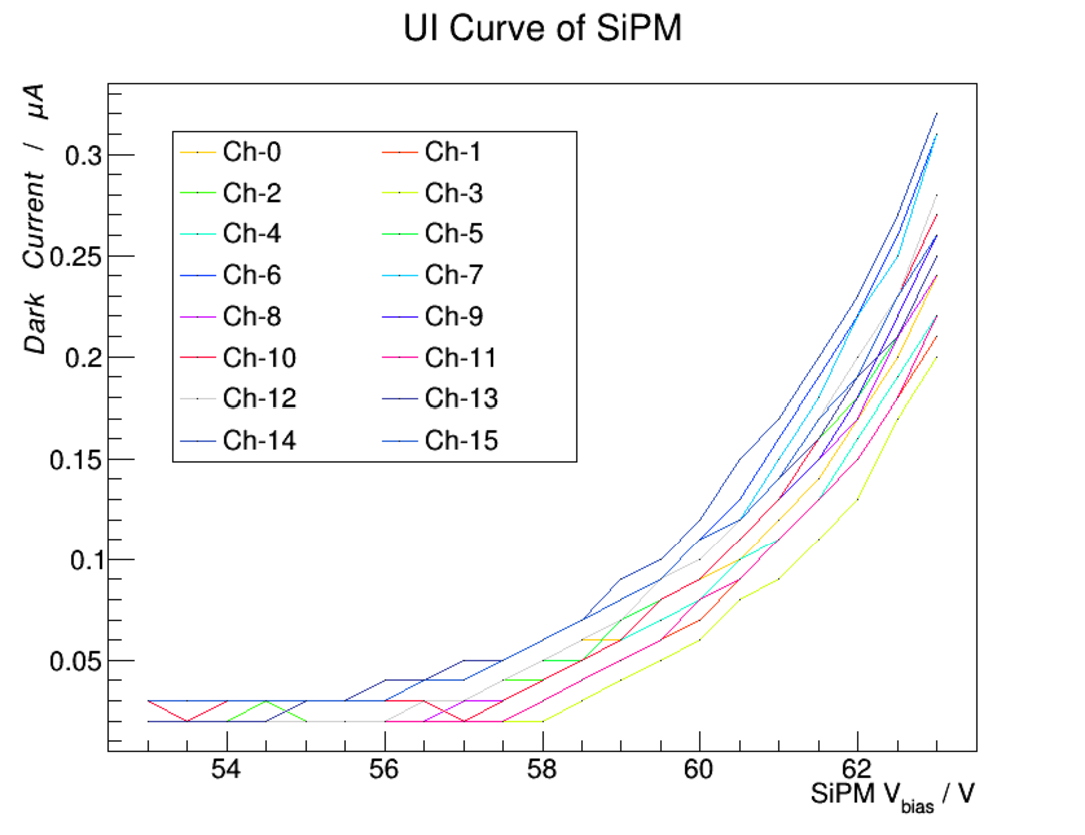
\includegraphics[scale=0.4]{fig/UI_Curve.pdf}}

    \end{floatrow}
    % \includegraphics[scale=0.25]{Flow_Chart.png}
\end{figure}



\section{SiPM Characterization}
    \paragraph{UI Curve}
    %we measure UI characteristic curve of each SiPM through current and voltage monitors, which are installed on FEE Boards. 
    
    % \begin{figure}[!h]
    %     \centering
    %     \graphicspath{{/Users/john/Desktop/EPD_Summary/UI_Curve/}}
    %     \includegraphics[scale=0.2]{Characteristic_UI_Curve_Example.jpg}
    %     \caption{UI Curve Example}\label{fig:UI Curve Example}
    % \end{figure}
    Typical UI curve of SiPM is like figure \ref{fig:UI Curve Example}, which shows UI curves of all 16 SiPMs in one FEE board.
    
    Due to low accuracy of current monitor, current measurement is less precise than 0.01$\mu$A.
    Thus, we can only get dark current quite roughly. Anyway, we can see a sudden increase when bias voltage increase.
    We choose the point, whose current is closest to 0.1 $\mu$A as break point, for the purpose of simplifing.
    At last, we can get distribution of "break down voltage".
 

    \paragraph{Noise} Comparison between oscilloscope and digitizer is showed in figure \ref{fig:Noise Comparison}
    % \begin{figure}[!h]
    %     \graphicspath{{/Users/john/Desktop/EPD_Summary/Noise/}}
    %     \ffigbox[\FBwidth]{}{
    %         {
    %             \begin{subfloatrow}[2]
    %                 \ffigbox[\hsize]{\caption{Oscilloscope noise}}{\includegraphics[scale=0.15]{Characteristic_Osc_Noise.jpg}}
    %                 \ffigbox[\hsize]{\caption{Electronic noise analysed by oscilloscope}}{\includegraphics[scale=0.15]{Characteristic_Noise_Osc.jpg}}
    %             \end{subfloatrow}    
    %         }
    %         \caption{Results from oscilloscope}\label{hello}
    %     }
    %     \ffigbox[\FBwidth]{}{{
    %     \begin{subfloatrow}[2]
    %         \ffigbox[\hsize]{\caption{Digitizer noise}}{\includegraphics[scale=0.15]{Characteristic_Dig_Noise.jpg}}
    %         \ffigbox[\hsize]{\caption{Electronic noise analysed by oscilloscope}}{\includegraphics[scale=0.15]{Characteristic_Noise_Dig.jpg}}
    %     \end{subfloatrow}}\caption{Results from digitizer}}


    %     % \end{floatrow}
    % \end{figure}

    \begin{figure}[ht]
        \centering
        \subfloat[Electronic Noise by Oscilloscope]{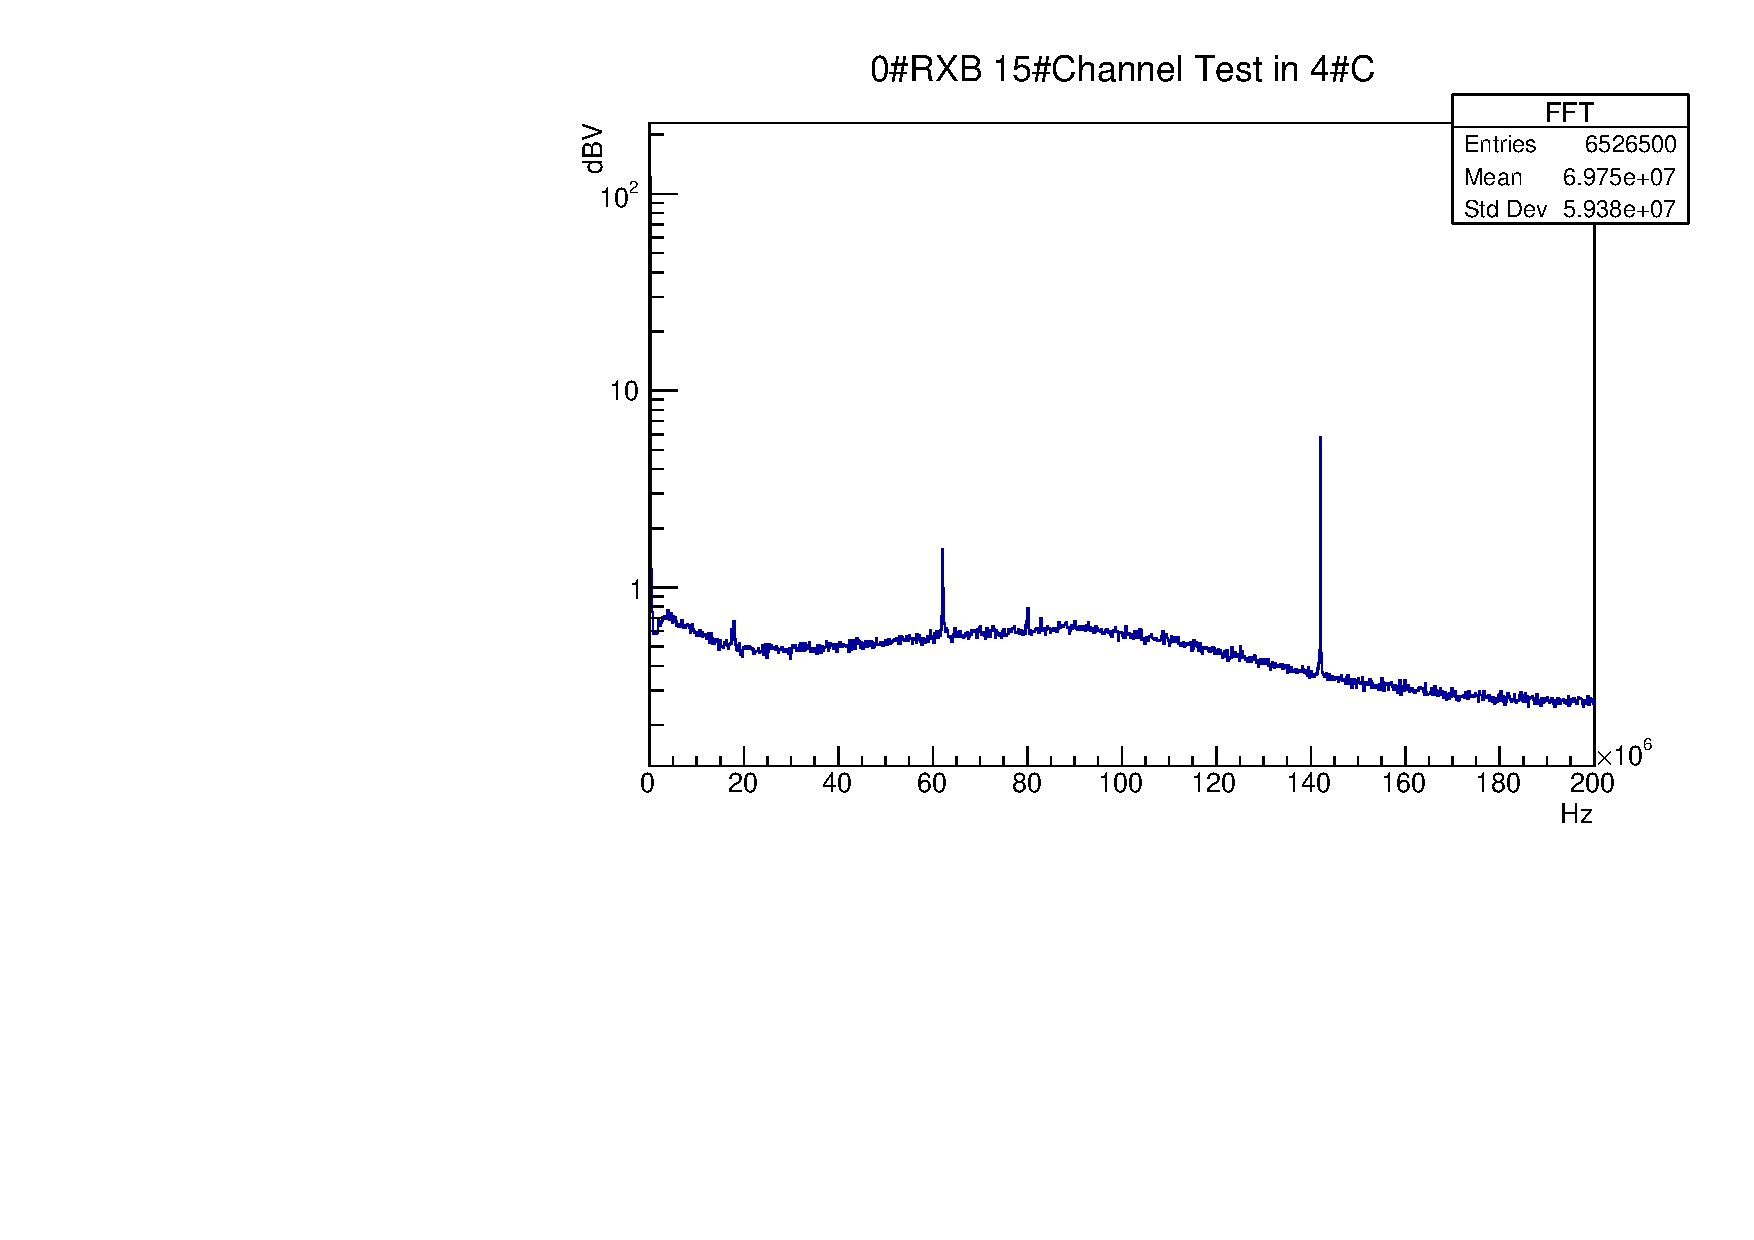
\includegraphics[scale=0.3]{fig/Noise_Osc.pdf}}\hspace{20pt}
        \subfloat[Electronic Noise by Digitizer]{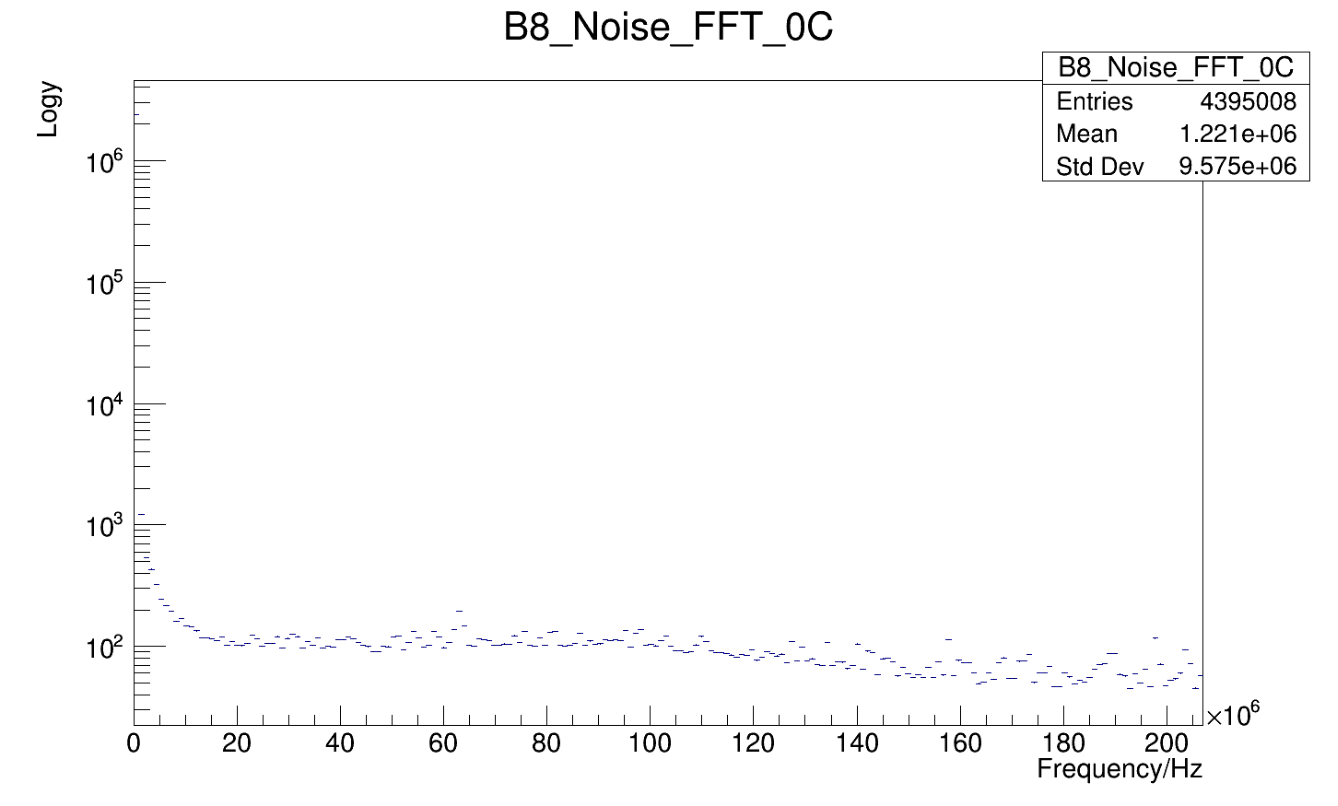
\includegraphics[scale=0.3]{fig/Noise_Dig.pdf}}\
        \subfloat[Oscilloscope Noise]{\includegraphics[scale=0.15]{fig/Osc_Noise.png}}
        % \subfloat[Digitizer Noise]{\includegraphics[scale=0.15]{_Dig_Noise.jpg}}\hspace{20pt}
        \caption{Comparison between Dig \& Osc}\label{fig:Noise Comparison}
    \end{figure}

    It seems that results from oscilloscope are more accuracy, while results from digitizer only have resolution of 1 MHz.
    Strangely, there still exist several ribs in oscilloscope noise spectrum when no signal input at all.
    We believe it's blame to oscilloscope itself.
    Considering of tight schedule, we deside to use digitizer to setup batch test system.
        
        % \centering
        % \includegraphics[scale=0.2]{Characteristic_Noise_Osc.jpg}
        % \caption{Noise spectrum measured by oscilloscope}

        % \includegraphics[scale=0.2]{Characteristic_Noise_Dig.jpg}
        % \caption{Noise spectrum measured by digtizer}
    % \end{figure}


    \paragraph{Signal}
    \begin{figure}
        \centering
        % \subfloat[Signal from Oscilloscope]{
            \ffigbox[\FBwidth]{}
            {
                {
                    \begin{subfloatrow}[2]
                        \ffigbox[\FBwidth]{\caption{Signal from Oscilloscope}}{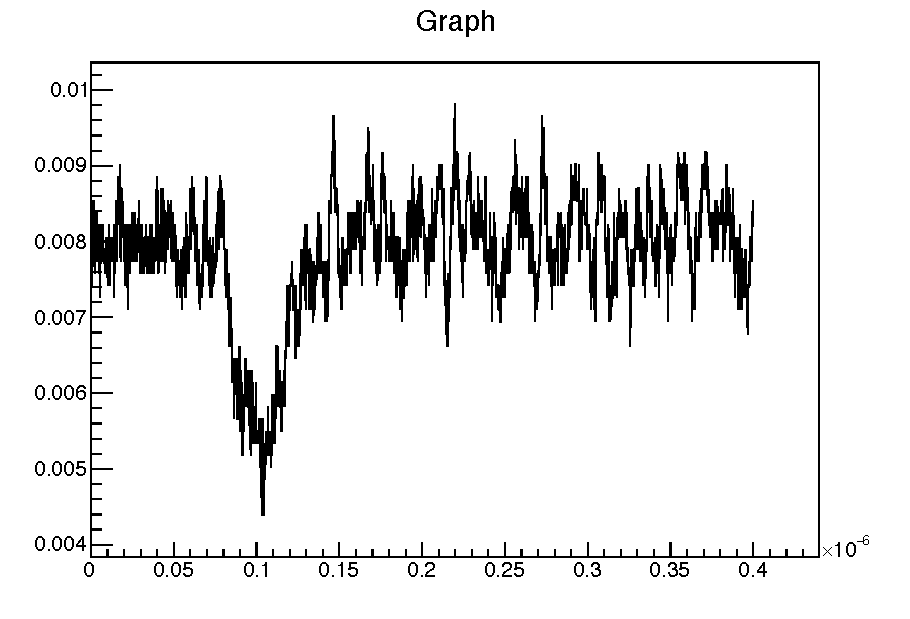
\includegraphics[scale=0.45]{fig/Signal_Osc2.pdf}}
                        % \ffigbox[\FBwidth]{\caption{Signal Persistence}}{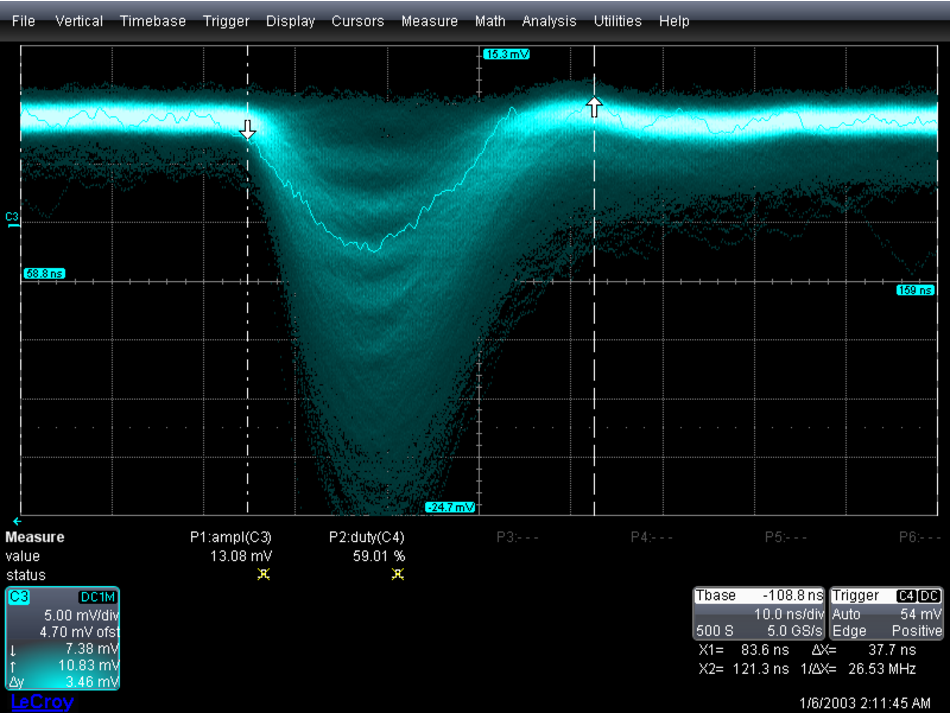
\includegraphics[scale=0.2]{Signal_Osc.pdf}}\
                        \ffigbox[\FBwidth]{\caption{Signals from Digitizer}\label{fig:Digitizer signal example}}{\includegraphics[scale=0.35]{fig/Signal_Dig.pdf}}
                    \end{subfloatrow}
                }
                \caption{Signal Examples}\label{fig:Signal Example}

            }
        % }
        % \subfloat[Signal from Digitizer]{\includegraphics[scale=0.2]{Signal_Dig.pdf}}

        % \caption{Signal Examples}\label{fig:Signal Example}

        % 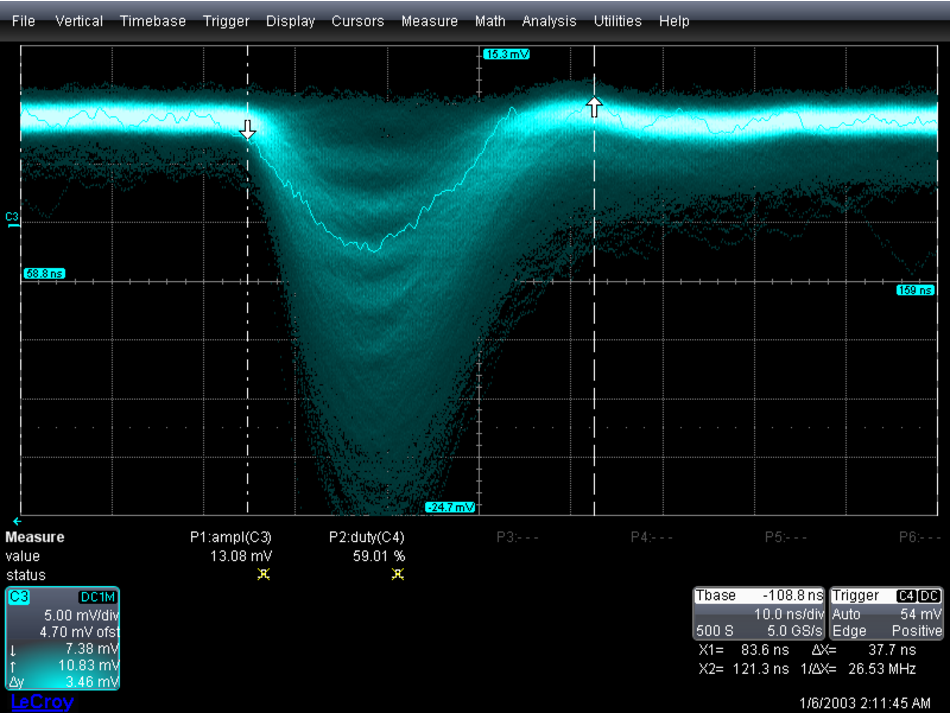
\includegraphics[scale=0.2]{Signal_Osc.pdf}
        % \caption{Signal Example}\label{fig:Signal Example}
    \end{figure}
    Signal examples are as shown in figure \ref{fig:Signal Example}.

    \subparagraph{Pedestal}As is shown in figure \ref{fig:Digitizer signal example}, pedestals of signals from digitizer are sloping.
    With further disicussion, we find that different pedestals have different slope.
    However, differece of slopes are too small to influnce pedestal value.
    Thus, it's a reasonable convention that average value of pedestal is its measurement result.

    \begin{figure}[ht]
        % \ffigbox[\FBwidth]{}{
        %     {
        %         \begin{subfloatrow}[2]
        %             \ffigbox{\caption{Result from oscilloscope}}{\includegraphics[scale=0.2]{Oscilloscope_Pedestal.jpg}}
        %             \ffigbox{\caption{Result from digitizer}}{\includegraphics[scale=0.2]{Digitizer_Pedestal.jpg}}
        %         \end{subfloatrow}
        %     }

        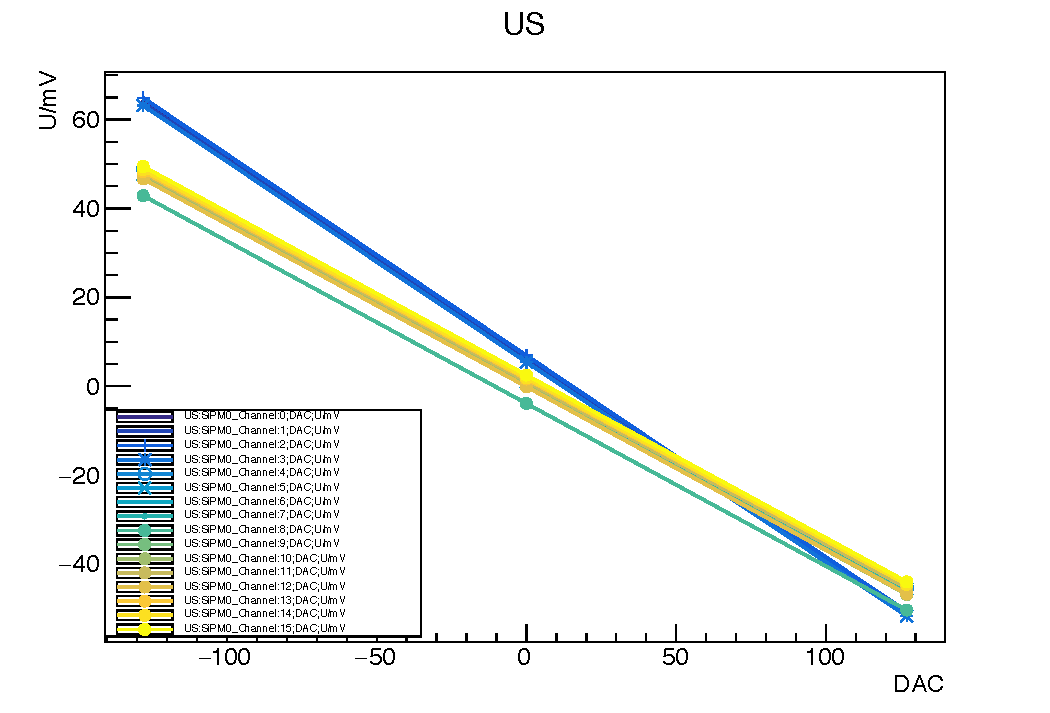
\includegraphics[scale=0.5]{fig/Pedestal.pdf}
        \caption{Pedestal Testing}\label{fig:Pedestal Testing}
        % }
    \end{figure}


    % Figure \ref{fig:Pedestal Testing} shows relation between DAC and pedestal value. We can see that DAC can work well.
    From figure \ref{fig:Pedestal Testing} we can see adjusting range of pedestal.





    \subparagraph{Charge Intergral of Signal}

    We collect more than 5000 signals from oscilloscope/digitizer and then integrate time and amplitude. Finally, we get its
    spectrum like figure \ref{fig:Integral Testing}.

    There's a little trick when analysing waveforms from digitizer. Assuming the signal interval that contains whole SiPM signals activated
    by photons from LED is 550ns to 650ns.
    We choose 430ns and 530ns as our first reference interval, and 670ns to 770ns as second reference interval. 
    Average of this two reference intervals can be regard as pedestal value of signal interval's midpoint.
    Minusing the average value when integrating can totally get rid of influnce of pedestal slope, and increase resolution of photon spectrum.

    Furthermore, we need to abandon waveforms which contain signal in reference intervals. It's easy to do that if we compare the slope, which is 
    calculated by two average value of two intervals, with the distribution of slope. If the calculated slope is far away from mean value of 
    pedestal distribution, this waveform should be dump.

    \begin{figure}[ht]
        \ffigbox[\FBwidth]{}{
            {
                \begin{subfloatrow}[2]
                    \ffigbox{\caption{Result from oscilloscope}}{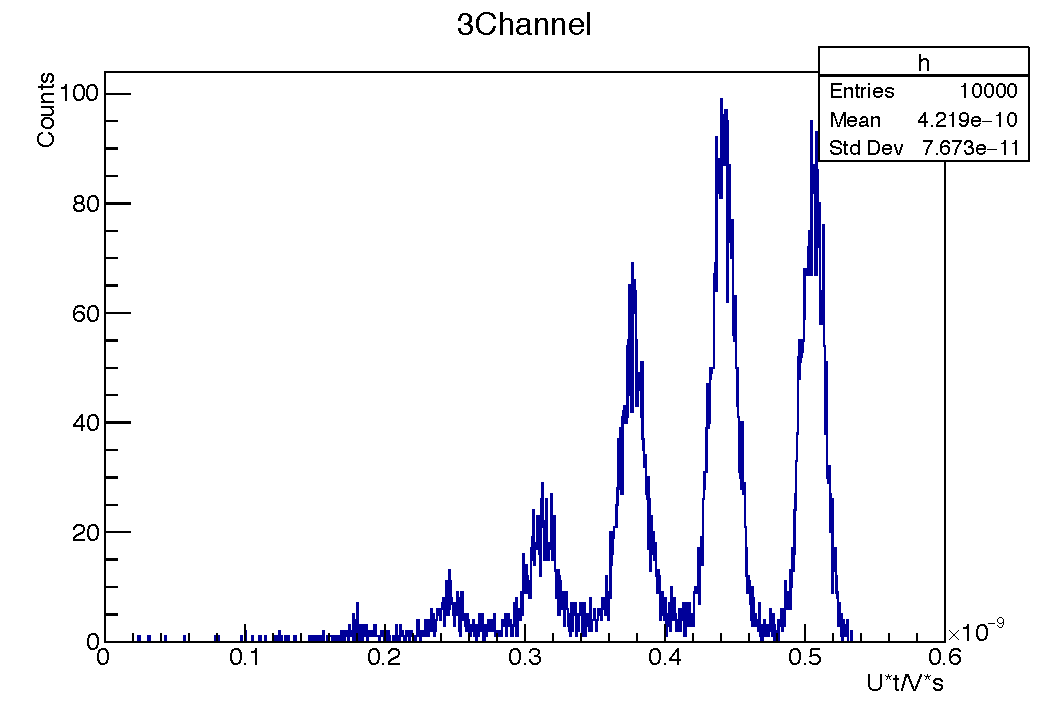
\includegraphics[scale=0.4]{fig/Oscilloscope_Integral.pdf}}
                    \ffigbox{\caption{Result from Digitizer}}{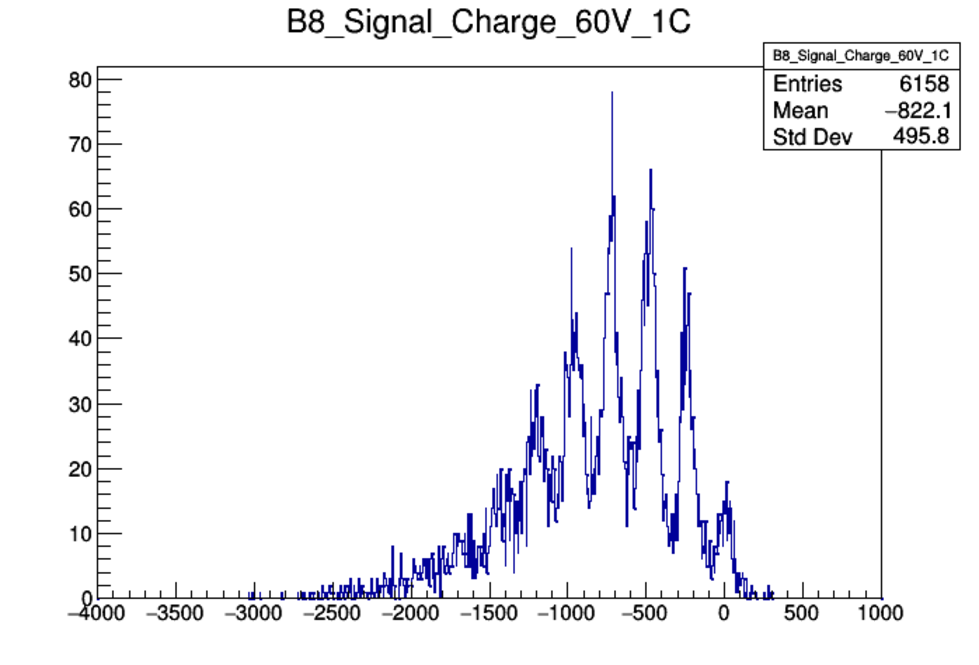
\includegraphics[scale=0.4]{fig/Digitizer_Integral.pdf}}
                \end{subfloatrow}
            }
            \caption{Integral Testing}\label{fig:Integral Testing}
        }
        % \includegraphics[scale=0.2]{Integral_Example.jpg}
        % \caption{fjldksajf}
    \end{figure}

    
    % \begin{figure}[ht]
    %     \graphicspath{{/Users/john/Desktop/EPD_Summary/Signal/Integral/}}
    %     \centering
    %     \includegraphics[scale=0.2]{Dig_Signal_Process.jpg}
    %     \caption{Process signal from digitizer}
    % \end{figure}

    



\section{Batch Test}
% \paragraph{Digitizer Calibration}Due to tight time schedule, we decide to use digitizer instead of oscilloscope.
% However, calibration of digitizer should be done before we setup batch test system.
% Have pulse generator generated pulses with different amplitudes. And output them seperately to digitizer and oscilloscope.
\section{Summary}
% \subsection{}


\end{document}
